\documentclass[11pt]{article}
%\documentclass[twocolumn, trackchanges]{aastex62}

\usepackage{hyperref}
\usepackage{longtable}
\usepackage{color}
\usepackage{graphics}
\usepackage{graphicx}

%Gummi|065|=)
\title{ULIRG reduction steps}

\date{}
\begin{document}
\maketitle

\tableofcontents


\section{Steps of analysis}

\begin{itemize}
\item Download data for ULIRGs from \url{http://archive.stsci.edu/hst/search.php} with project id 13655.

  
\end{itemize}
\begin{center}
\input{/home/sourabh/ULIRG_v3/notebooks/cont_flt_latex.tex}
\end{center}

\subsection{Dark and sky subtraction}

\begin{itemize}
	\item We work with `FLT' images in this process. Because we want to avoid noise arising from drizzling process.
	\item We assume that the spatial structure observed in the galaxy frame other than the main galaxy itself originates from the dark current. We start by considering all the 20 dark exposures and select the dark exposure based on our minimization process. The image frame and corresponding dark frames should differ only by a scaling factor, which is a function of exposure time and the temperature of the detector ($A^T_{Exp}$). In addition to $A^T_{Exp}$, we also include a constant $K$, which takes care of sky subtraction in the image. We assume that the sky value is a constant and there is no spatially varying sky.
	\item In order to remove the contribution from galaxy itself, we find a circular radii $R_{95}$ \footnote{Radius at which the total flux falls to 95$\%$  of the total flux} of the galaxy by following these steps:-
	\begin{itemize}
		\item First, we subtract a constant sky value from one of the F125LP frames.
		\item Next, we find the brightest pixel in one of the F125LP frames. 
		\item Then we perform aperture photometry with circular apertures to find out the radius at which the total flux in the exposure falls to 95$\%$  of the total flux of the galaxy.
		\item We mask a circular region on the image centered at pixel position (512, 512) and radius that covers the $R_{95}$
	\end{itemize}  We mask a circular region on the image centered at central pixel of SBC filed of view (i.e. (512, 512)) and radius that covers $R_{95}$ radius of the galaxy. For all the following analysis, we work with the masked image of the galaxy. We mask the same region in dark exposures.

	 \item Out of 20 dark exposures, we select the best dark, by identifying the scaling factor and sky value that minimizes the aperture photometric residuals between the image frame and the scaled dark frame. 
\end{itemize}


In the following, we explicitly write the scaling factor as the product of two terms:

\begin{equation}
A^T_{Exp} = A^T*A_{Exp} = A^T*\frac{exp_{gal}}{exp_{dark}}
\end{equation}

where, $A^T$ depends on the detector temperature only, and $\frac{exp_{gal}}{exp_{dark}}$ accounts for the different exposure times (which are known). We find $A^T$ and $K$ by minimizing the residual between the fluxes in the scaled dark exposures and the galaxy image.  
\begin{equation}
  f_g^{out}(i,j)  = f_{g}^{in}(i,j) -  A^T*\frac{exp_{gal}}{exp_{dark}} * f_{dark}^{k}(i, j) - K
 \end{equation}

Where $f_{g}^{in}(i,j)$, $f_{g}^{out}(i,j)$, $f_{dark}^{k}(i, j)$ are counts at pixel position (i,j) in the input and output galaxy images and $k^{th}$ dark exposure. $A^T$ and $K$ are the parameters that are to be determined using minimization process. There is a total of 20 dark exposures so $k\in[1,20]$. 


Minimization of the residuals of two images i.e. using minimizing function as $$F[A^T, k, K] = \sum_{i,j}(f_{g}^{out}(i,j)[A^T, k, K])^2$$ does not work as the distribution of pixels with non-zero counts are is very sparse which leads to minimum value of $A^T$ and $K$ as zeros. Therefore, we use a minimizing function\footnote{Refer to appendix A} dependent on radial variation. 
\begin{equation}
\label{eq:min}
G[A^T, k, K] = \sum_{r<r_0} |f_g^{out}(r)|
\end{equation}
where
\begin{equation}
f_g^{out}(r) = \frac{1}{2\pi r \Delta r}\sum_{(i, j) : r_{i,j} \in [r-\Delta r/2<,r+\Delta r/2]} f_g^{out}( i-i_0, j -j_0)
\end{equation}




\begin{figure*}
 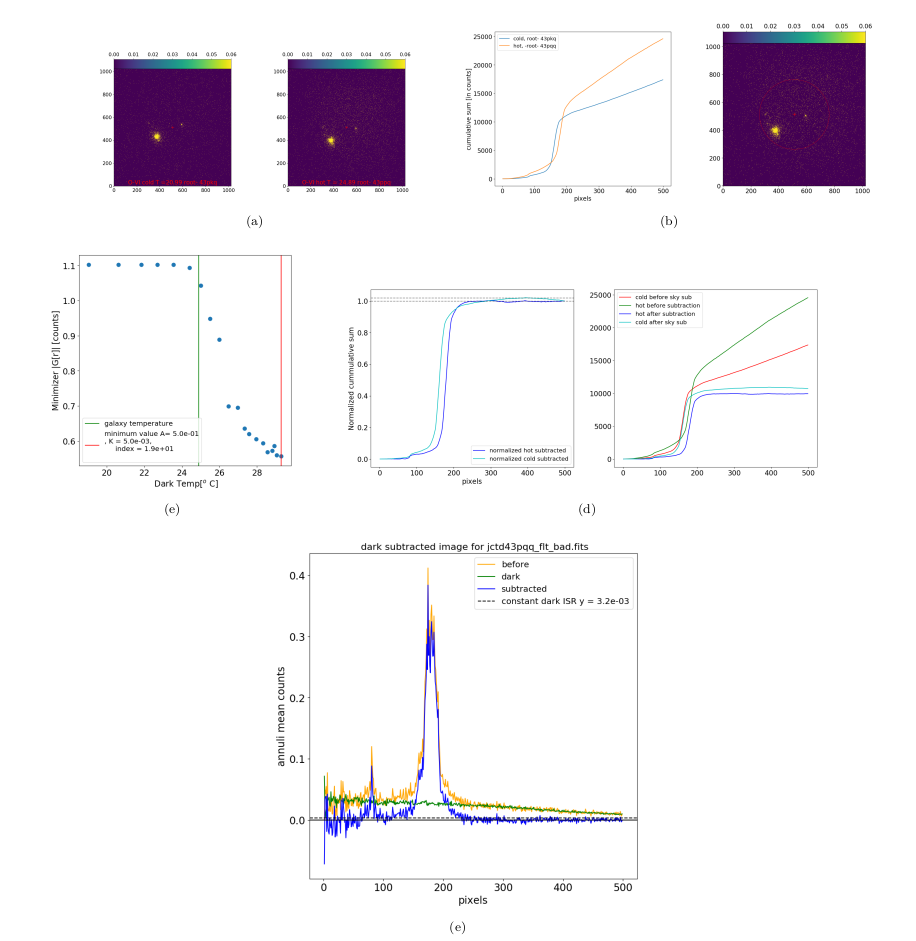
\includegraphics[scale=0.40]{dark_sub.png}

\caption{The figure shows the results of applying the dark subtraction method to a sample image
(a) Two cold and hot frames. We correct for dark subtraction in hot frame., (b) Cumulative sum profile for FLT files at two different temperature. (c) Minimizer value as a function of temperature of darks (d) Dark subtracted cumulative radial profiles for hot frame before and after subtraction, (e) Radial profile for galaxy in circular apertures centered at (512, 512). \label{fig:O-VI}}
\end{figure*}



\begin{figure}
 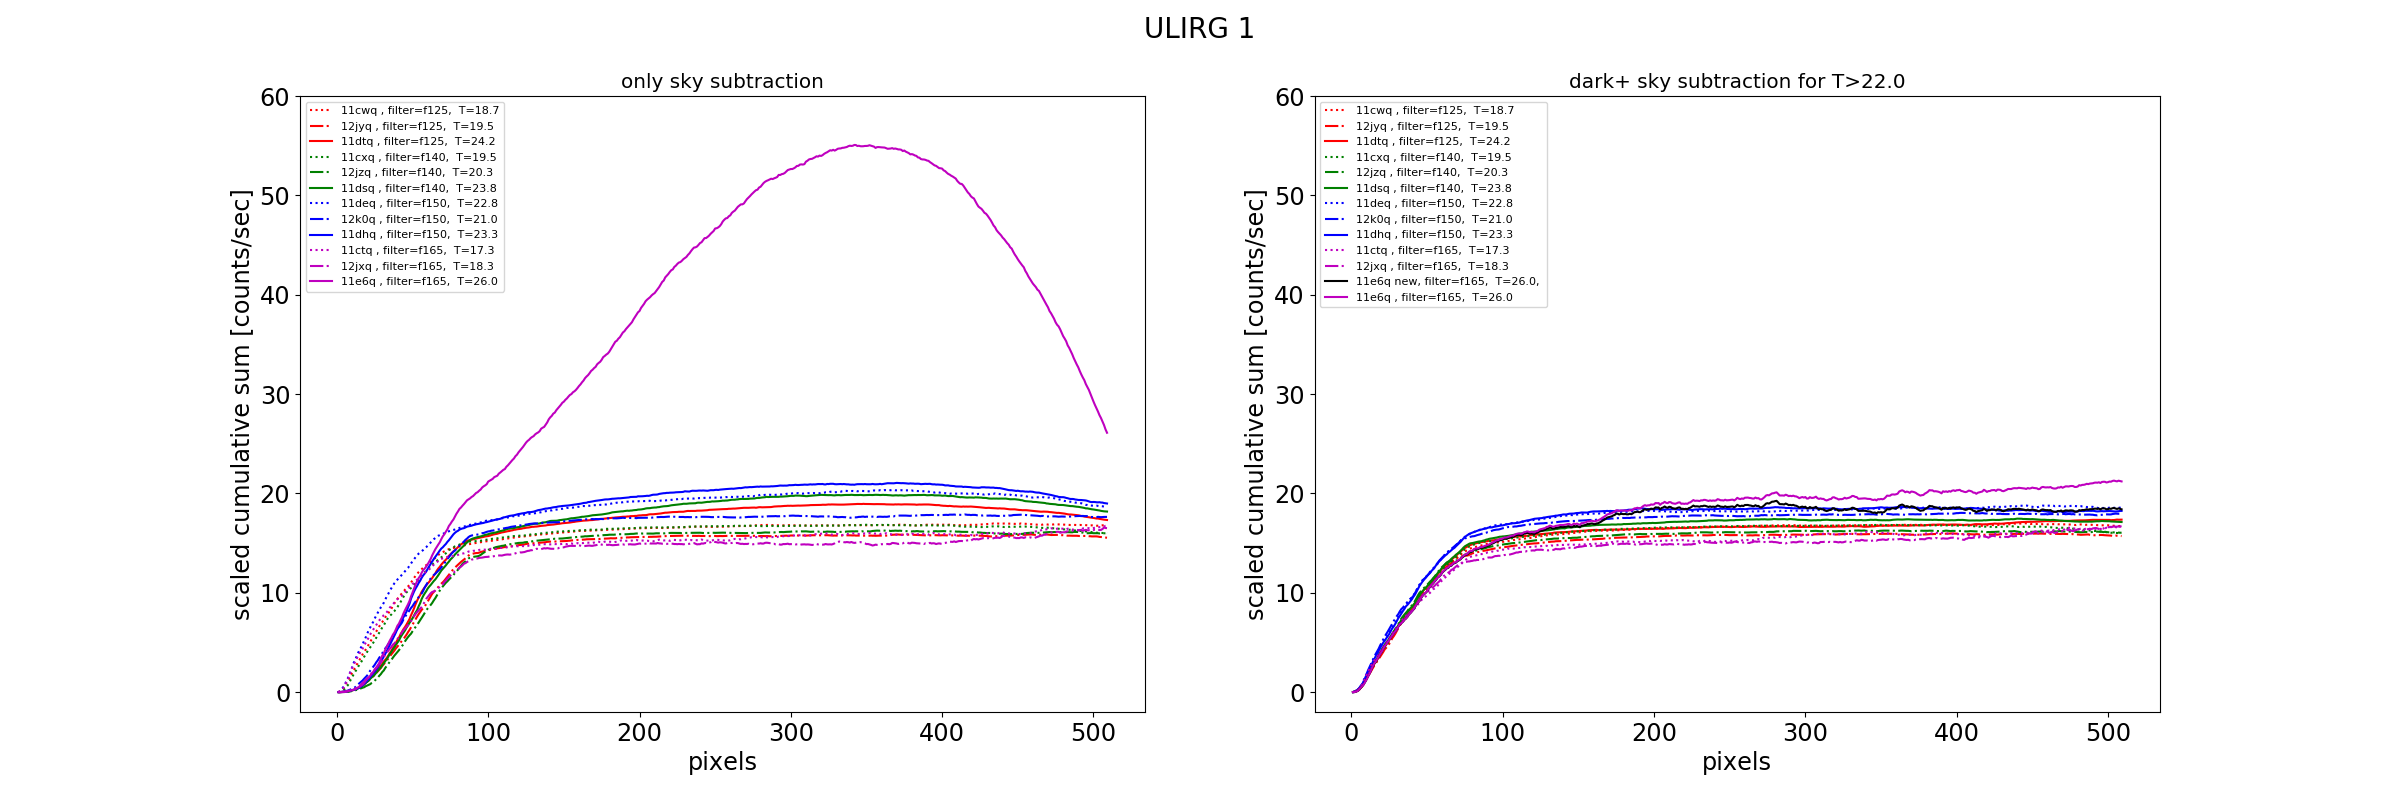
\includegraphics[scale=0.30]{gal1_photometry_FLT_subtracted_final.png}

\caption{The figure shows circular aperture photometry on each of the exposure for ULIRG 1 before and after sky+dark subtraction. \label{fig:gal1}
 }
\end{figure}

\begin{figure}
 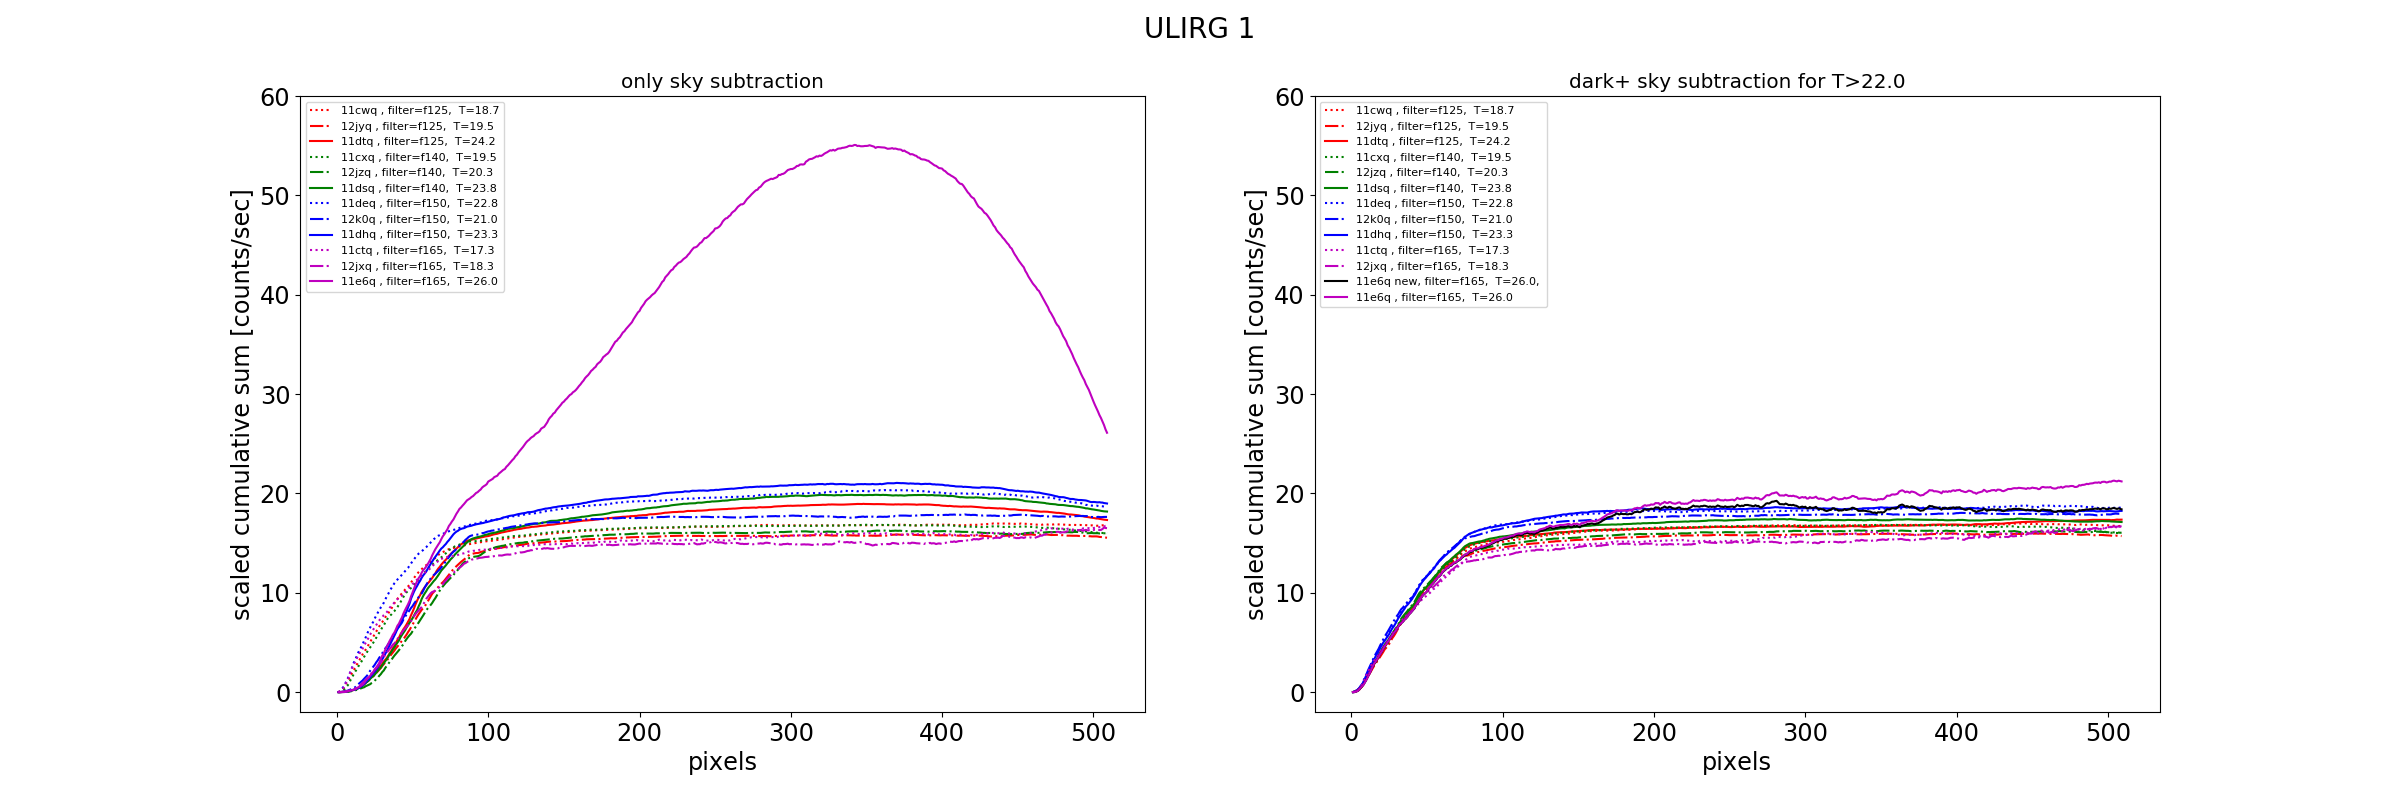
\includegraphics[scale=0.30]{gal1_photometry_FLT_subtracted_final.png}

\caption{The figure shows circular aperture photometry on each of the exposure for ULIRG 1 before and after sky+dark subtraction. \label{fig:gal1}
 }
\end{figure}
\begin{figure}
 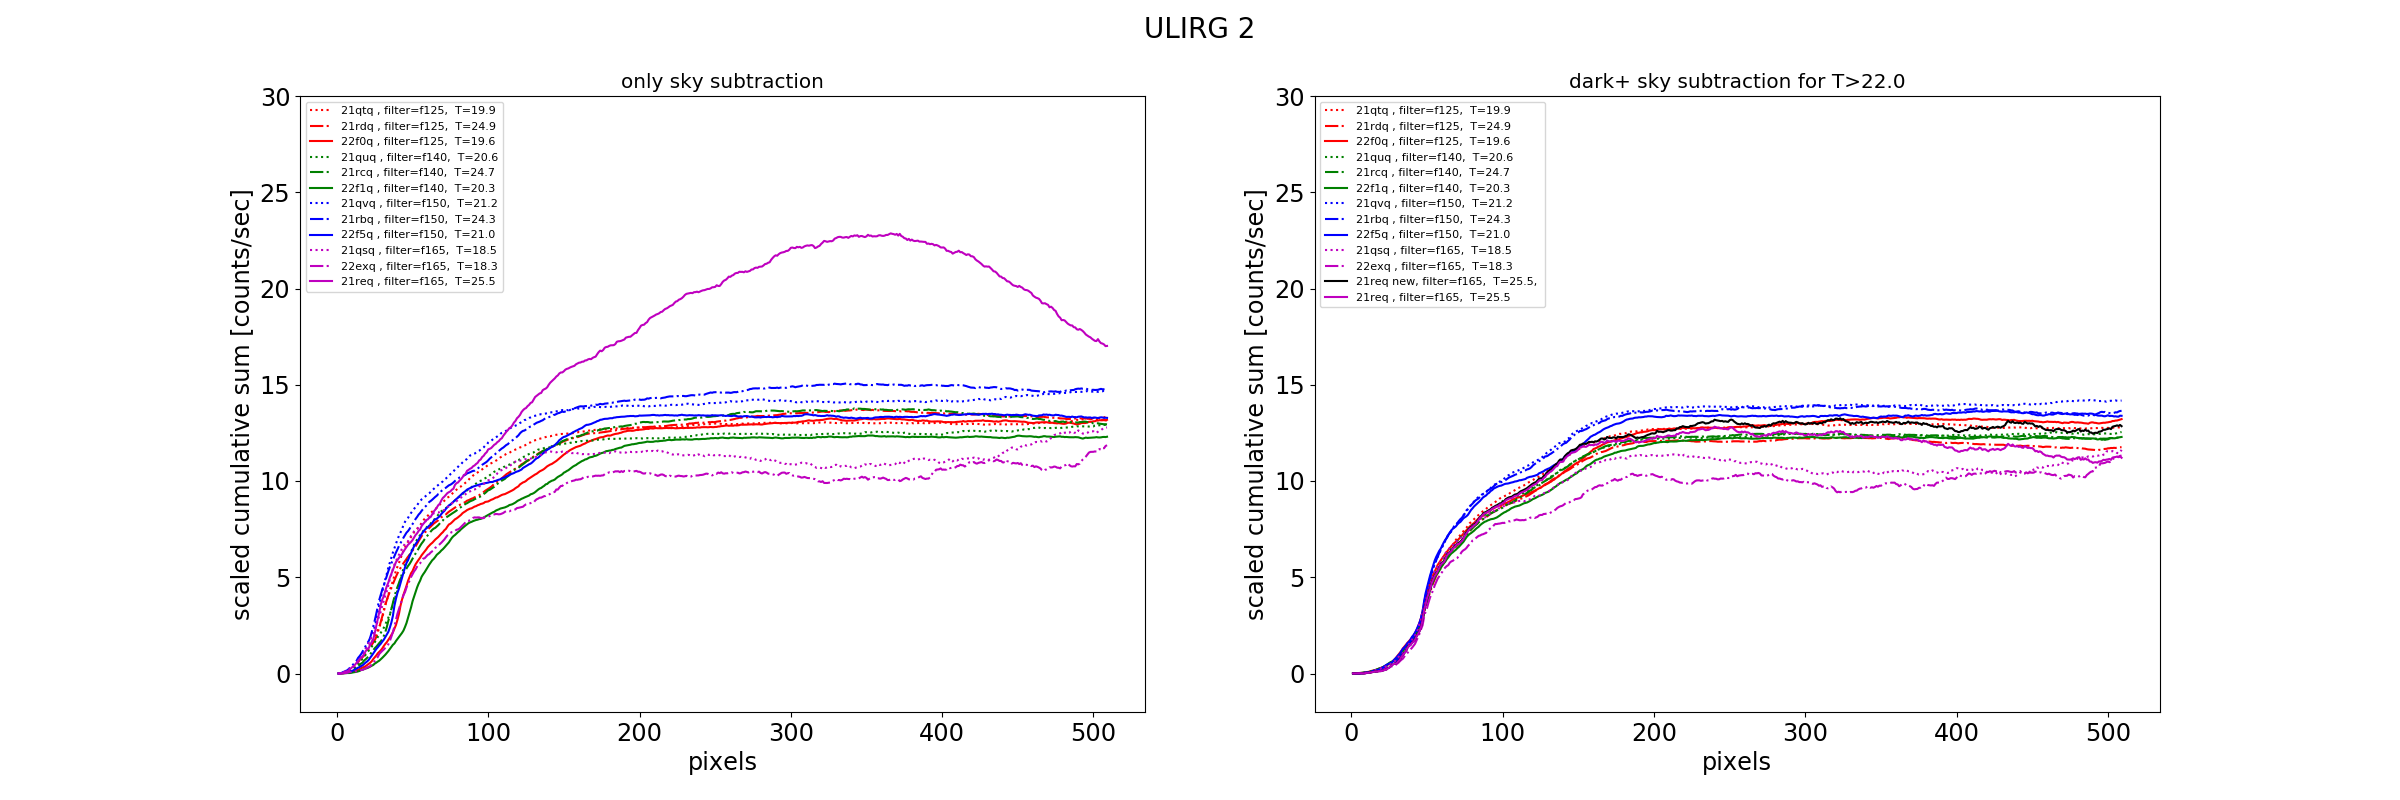
\includegraphics[scale=0.30]{gal2_photometry_FLT_subtracted_final.png}

\caption{The figure shows circular aperture photometry on each of the exposure for ULIRG 2 before and after sky+dark subtraction. \label{fig:gal2}
 }
\end{figure}
\begin{figure}
 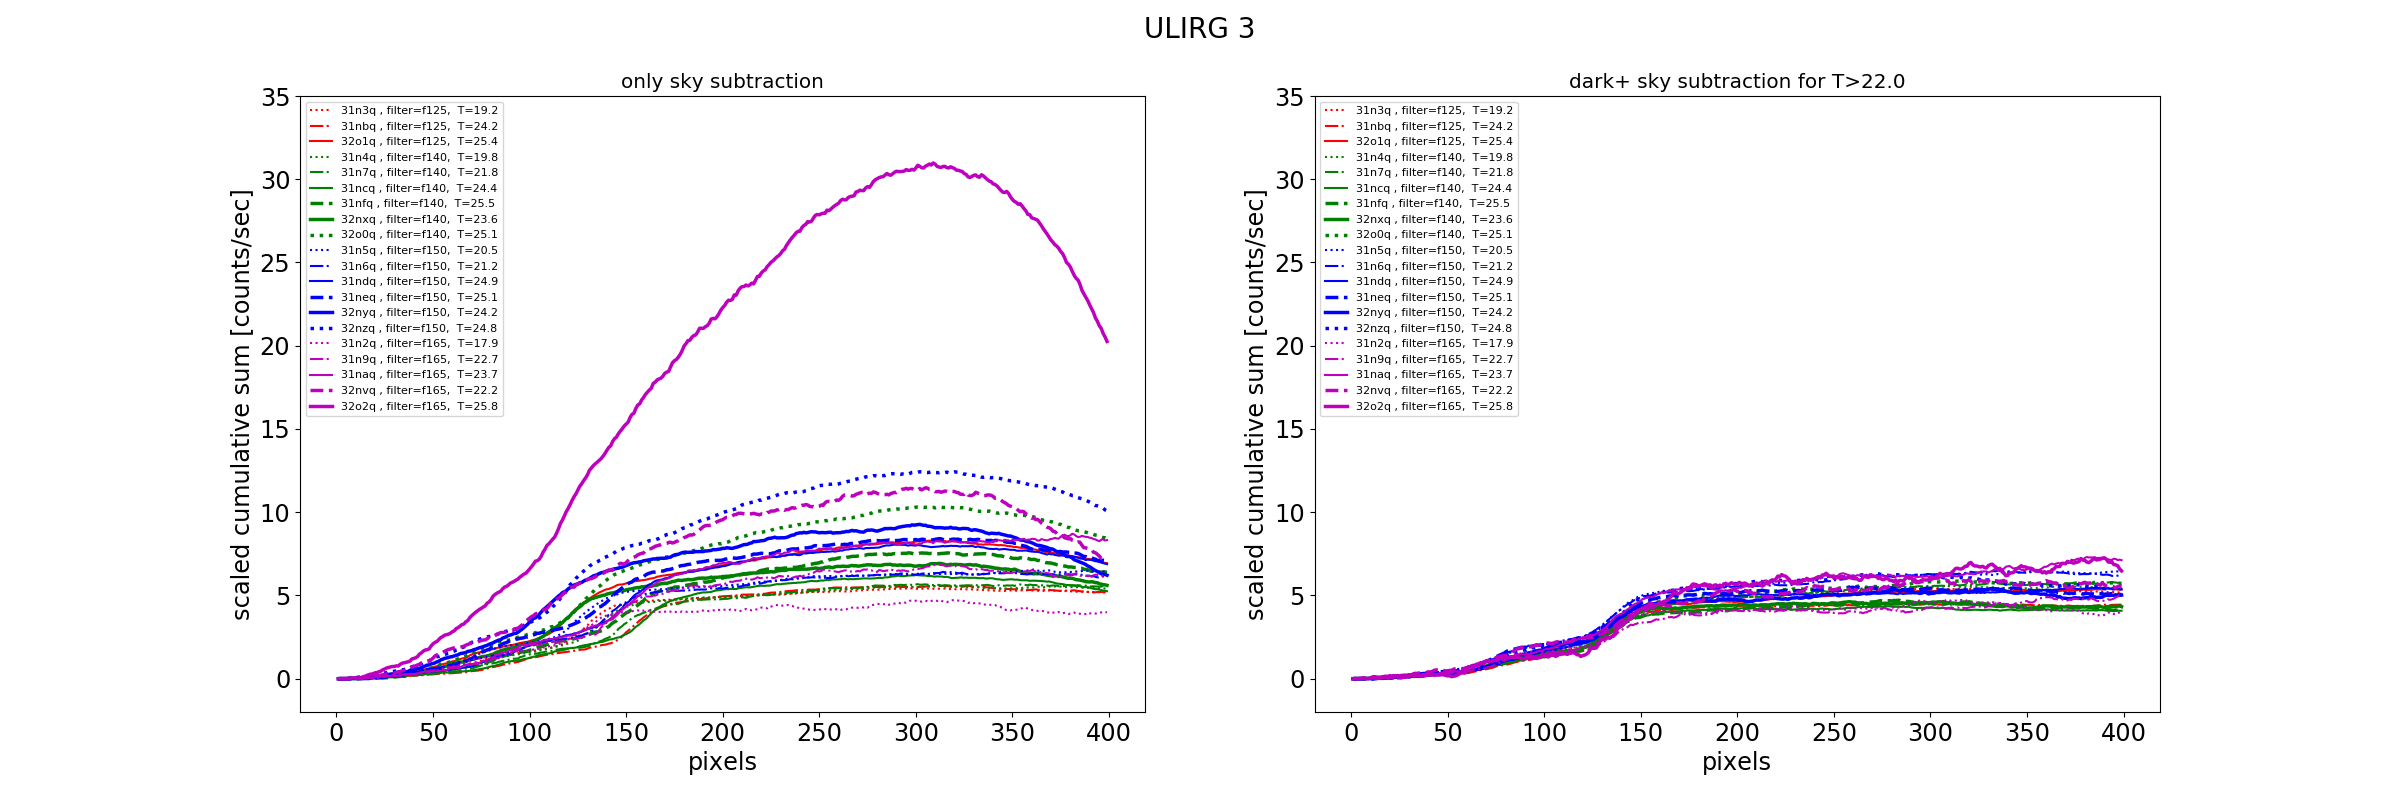
\includegraphics[scale=0.30]{gal3_photometry_FLT_subtracted_final.png}

\caption{The figure shows circular aperture photometry on each of the exposure for ULIRG 3 before and after sky+dark subtraction. \label{fig:gal3}
 }
\end{figure}
\begin{figure}
 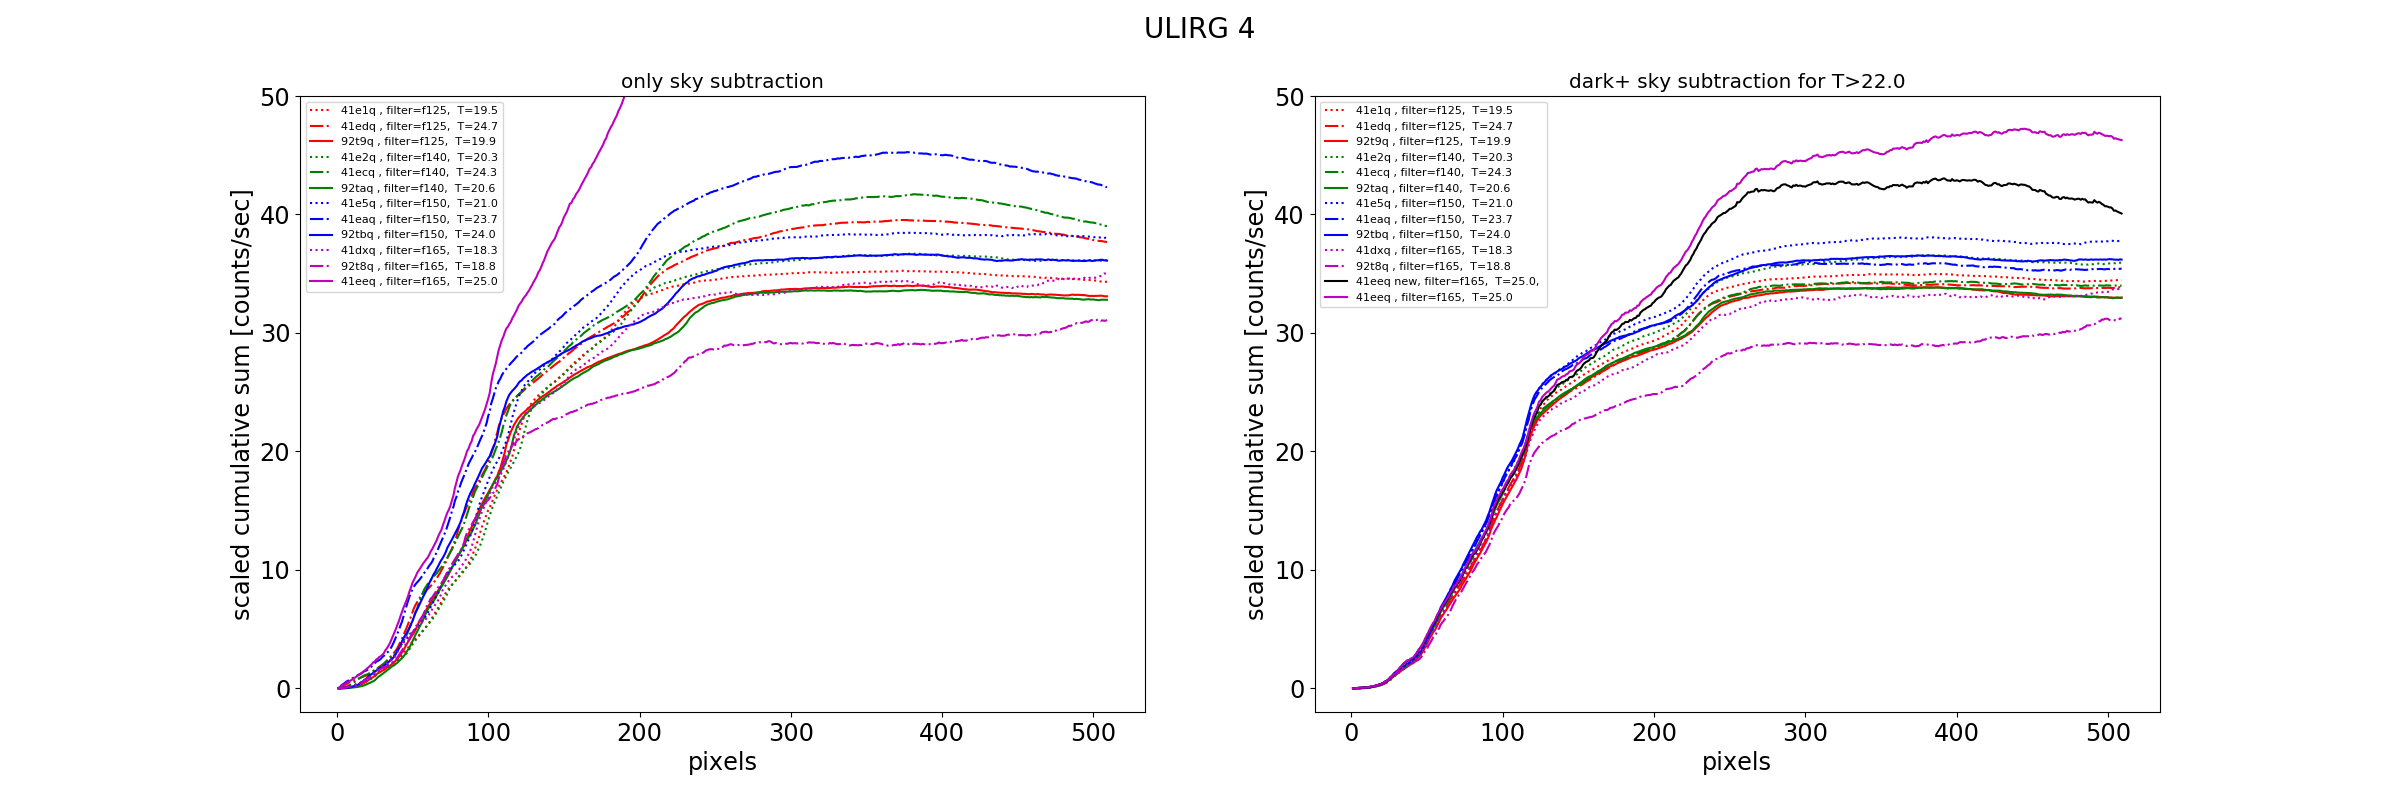
\includegraphics[scale=0.30]{gal4_photometry_FLT_subtracted_final.png}

\caption{The figure shows circular aperture photometry on each of the exposure for ULIRG 4 before and after sky+dark subtraction. \label{fig:gal4}
 }
\end{figure}

\begin{figure}
 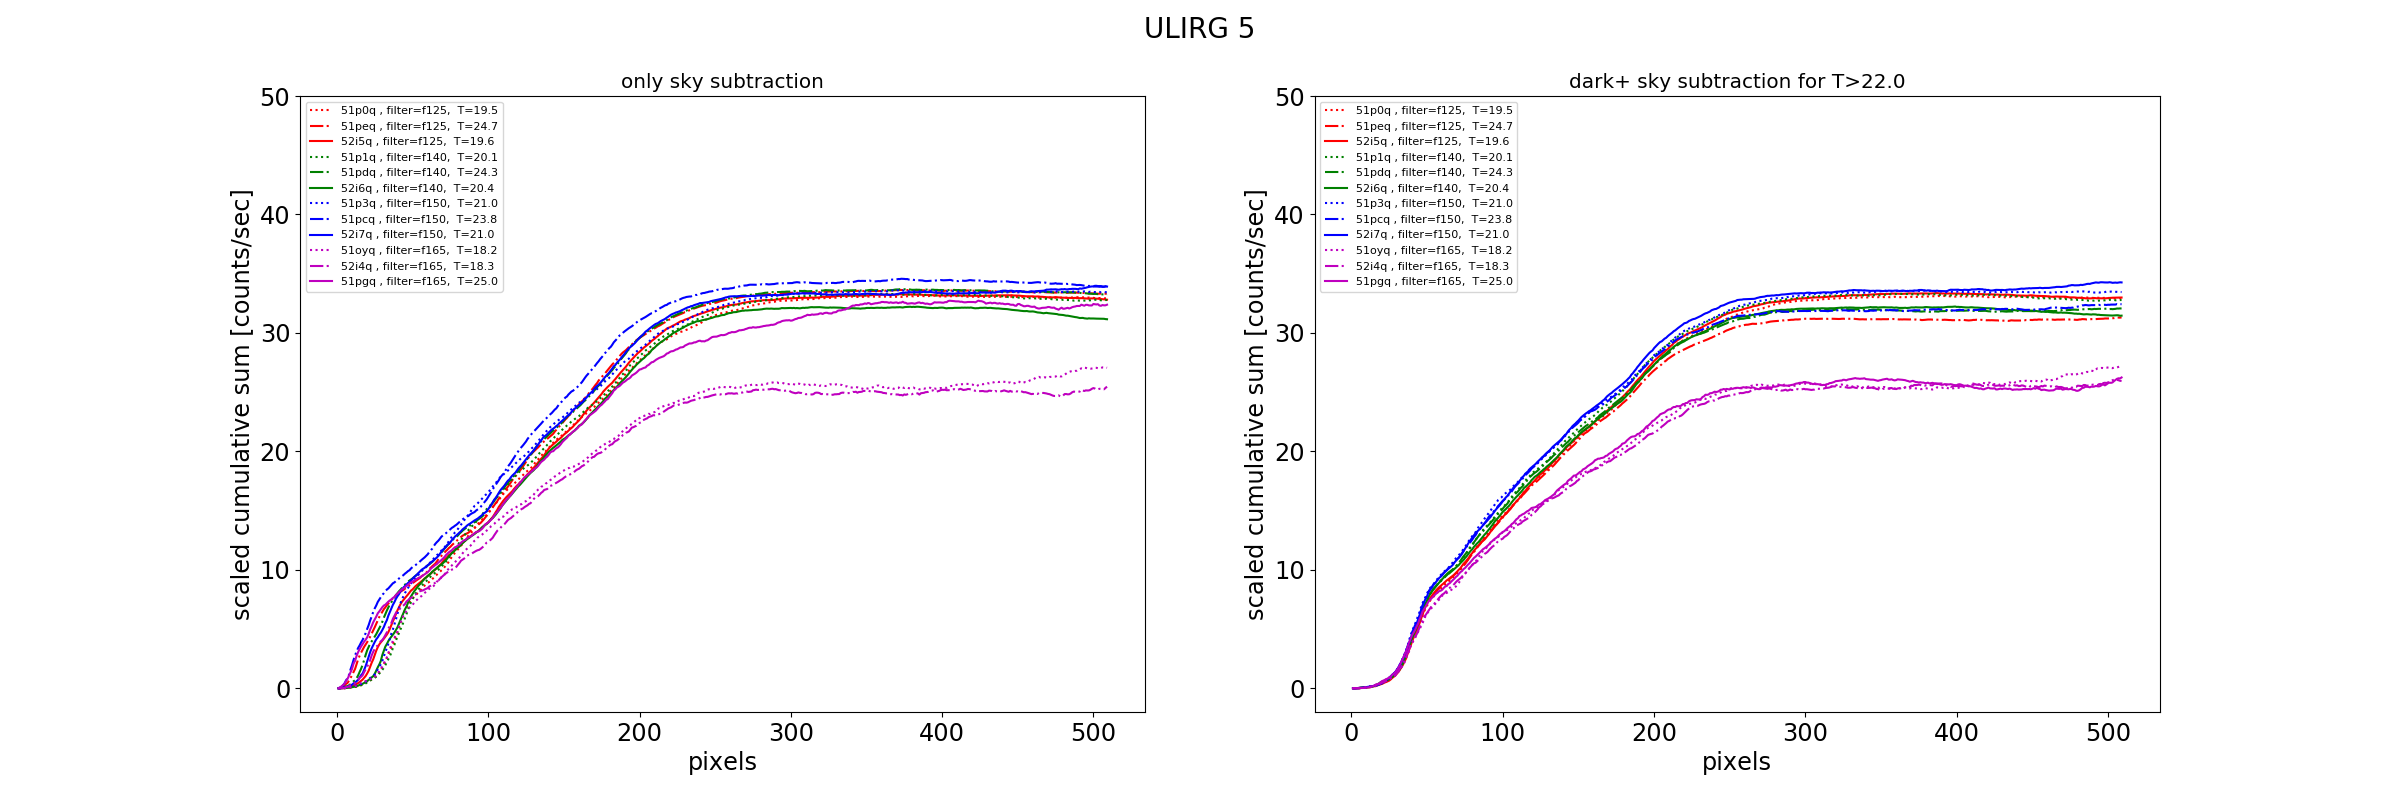
\includegraphics[scale=0.30]{gal5_photometry_FLT_subtracted_final.png}

\caption{The figure shows circular aperture photometry on each of the exposure for ULIRG 5 before and after sky+dark subtraction. \label{fig:gal5}
 }
\end{figure}
\subsection{Aligning FLT images}
As there are no point sources in the 

\subsection{Combining FLT files using astrodrizzle}
\begin{itemize}
	\item \textbf{INTERMEDIATE files}
	\item \textbf{parameters} 
	\item \textbf{Example command}
	\end{itemize}

\subsection{psfmatch}

\begin{itemize}
	\item \textbf{INTERMEDIATE files}
	\item \textbf{parameters} 
	\item \textbf{Example command}
	\end{itemize}

\subsection{PHOTFLAM factor }

\begin{itemize}
	\item \textbf{INTERMEDIATE files}
	\item \textbf{parameters} 
	\item \textbf{Example command}
	\end{itemize}

\section{spectrum}
	



\end{document}
